\documentclass{standalone}
\usepackage{tikz}
\usetikzlibrary{patterns, positioning}


\begin{document}
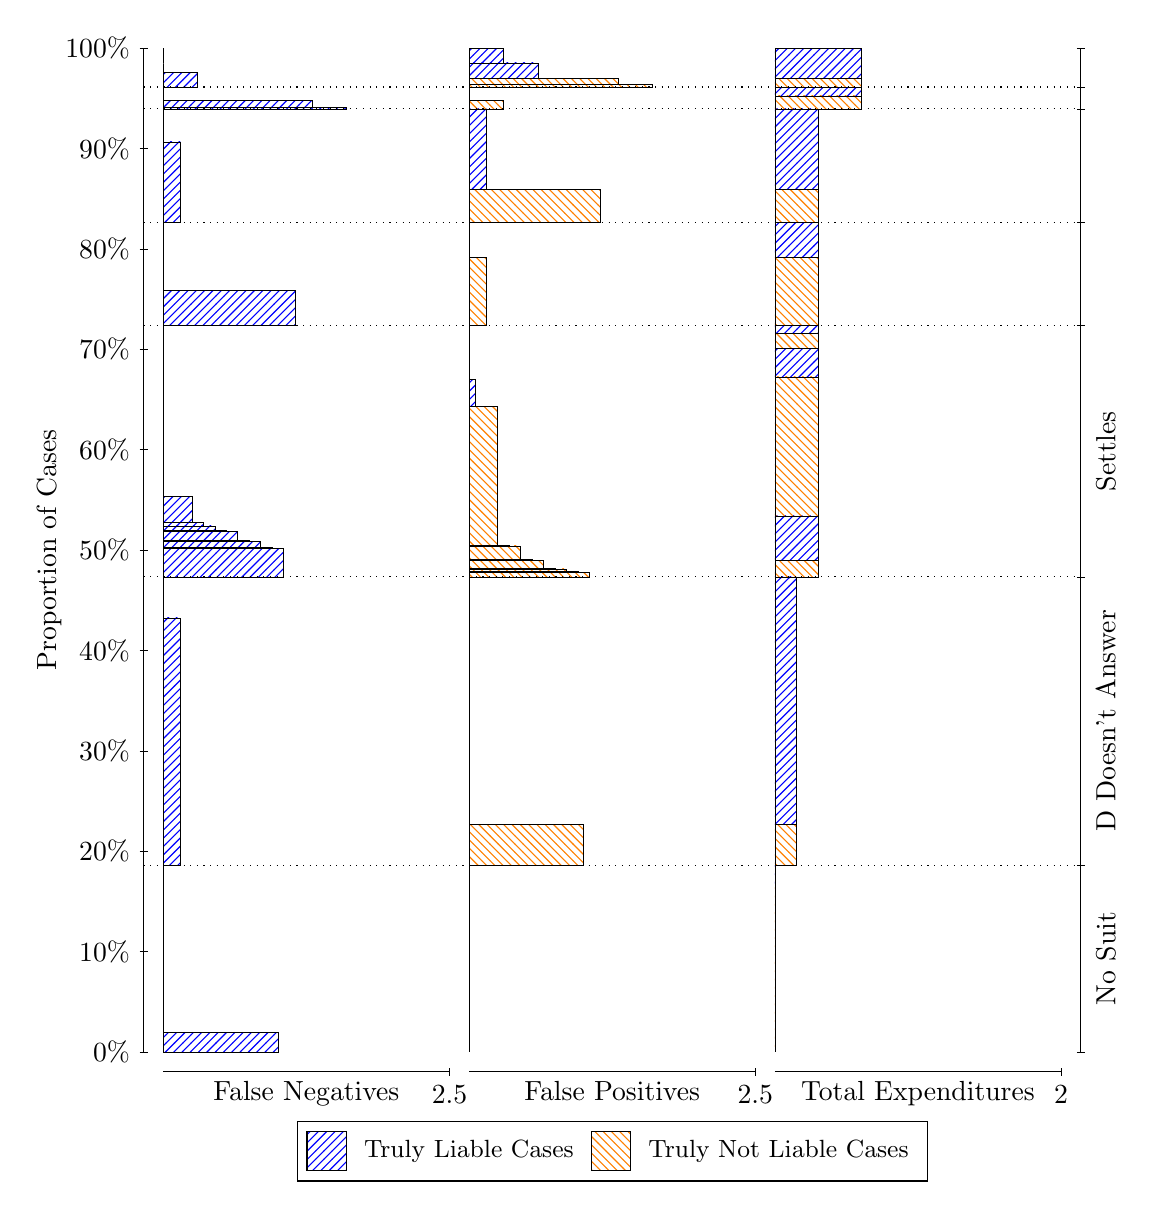
\begin{tikzpicture}
\draw[black, very thin] (1.5,1.75) -- (1.5,14.5);
\node[rotate=90, text=black, anchor=center] at (0.3, 8.125) {Proportion of Cases};
\draw[black, very thin] (1.45,1.75) -- (1.55,1.75);
\node[text=black, anchor=east] at (1.45, 1.75) {0\%};
\draw[black, very thin] (1.45,3.025) -- (1.55,3.025);
\node[text=black, anchor=east] at (1.45, 3.025) {10\%};
\draw[black, very thin] (1.45,4.3) -- (1.55,4.3);
\node[text=black, anchor=east] at (1.45, 4.3) {20\%};
\draw[black, very thin] (1.45,5.575) -- (1.55,5.575);
\node[text=black, anchor=east] at (1.45, 5.575) {30\%};
\draw[black, very thin] (1.45,6.85) -- (1.55,6.85);
\node[text=black, anchor=east] at (1.45, 6.85) {40\%};
\draw[black, very thin] (1.45,8.125) -- (1.55,8.125);
\node[text=black, anchor=east] at (1.45, 8.125) {50\%};
\draw[black, very thin] (1.45,9.4) -- (1.55,9.4);
\node[text=black, anchor=east] at (1.45, 9.4) {60\%};
\draw[black, very thin] (1.45,10.675) -- (1.55,10.675);
\node[text=black, anchor=east] at (1.45, 10.675) {70\%};
\draw[black, very thin] (1.45,11.95) -- (1.55,11.95);
\node[text=black, anchor=east] at (1.45, 11.95) {80\%};
\draw[black, very thin] (1.45,13.225) -- (1.55,13.225);
\node[text=black, anchor=east] at (1.45, 13.225) {90\%};
\draw[black, very thin] (1.45,14.5) -- (1.55,14.5);
\node[text=black, anchor=east] at (1.45, 14.5) {100\%};

\draw[black, very thin] (13.4,1.75) -- (13.4,14.5);
\draw[black, very thin] (13.35,1.75) -- (13.45,1.75);
\node[anchor=west] at (13.35, 1.75) {};
\draw[black, very thin] (13.35,4.1224) -- (13.45,4.1224);
\node[anchor=west] at (13.35, 4.1224) {};
\draw[black, very thin] (13.35,7.7848) -- (13.45,7.7848);
\node[anchor=west] at (13.35, 7.7848) {};
\draw[black, very thin] (13.35,10.976) -- (13.45,10.976);
\node[anchor=west] at (13.35, 10.976) {};
\draw[black, very thin] (13.35,12.286) -- (13.45,12.286);
\node[anchor=west] at (13.35, 12.286) {};
\draw[black, very thin] (13.35,13.727) -- (13.45,13.727);
\node[anchor=west] at (13.35, 13.727) {};
\draw[black, very thin] (13.35,14.005) -- (13.45,14.005);
\node[anchor=west] at (13.35, 14.005) {};
\draw[black, very thin] (13.35,14.5) -- (13.45,14.5);
\node[anchor=west] at (13.35, 14.5) {};

\draw[black, very thin, pattern color=blue, pattern=north east lines] (1.75,1.75) rectangle (3.2033,1.9996);
\draw[black, very thin, pattern color=orange, pattern=north west lines] (1.75,1.9996) rectangle (1.75,4.1224);
\draw[black, very thin, pattern color=blue, pattern=north east lines] (1.75,4.1224) rectangle (1.968,7.2635);
\draw[black, very thin, pattern color=orange, pattern=north west lines] (1.75,7.2635) rectangle (1.75,7.7848);
\draw[black, very thin, pattern color=blue, pattern=north east lines] (1.75,7.7848) rectangle (3.276,8.1439);
\draw[black, very thin, pattern color=blue, pattern=north east lines] (1.75,8.1439) rectangle (3.1307,8.1535);
\draw[black, very thin, pattern color=blue, pattern=north east lines] (1.75,8.1535) rectangle (2.9853,8.2369);
\draw[black, very thin, pattern color=blue, pattern=north east lines] (1.75,8.2369) rectangle (2.84,8.2465);
\draw[black, very thin, pattern color=blue, pattern=north east lines] (1.75,8.2465) rectangle (2.6947,8.3601);
\draw[black, very thin, pattern color=blue, pattern=north east lines] (1.75,8.3601) rectangle (2.5493,8.3743);
\draw[black, very thin, pattern color=blue, pattern=north east lines] (1.75,8.3743) rectangle (2.404,8.4321);
\draw[black, very thin, pattern color=blue, pattern=north east lines] (1.75,8.4321) rectangle (2.2587,8.473);
\draw[black, very thin, pattern color=blue, pattern=north east lines] (1.75,8.473) rectangle (2.1133,8.8096);
\draw[black, very thin, pattern color=orange, pattern=north west lines] (1.75,8.8096) rectangle (1.75,10.976);
\draw[black, very thin, pattern color=blue, pattern=north east lines] (1.75,10.976) rectangle (3.4213,11.419);
\draw[black, very thin, pattern color=orange, pattern=north west lines] (1.75,11.419) rectangle (1.75,12.286);
\draw[black, very thin, pattern color=blue, pattern=north east lines] (1.75,12.286) rectangle (1.968,13.309);
\draw[black, very thin, pattern color=orange, pattern=north west lines] (1.75,13.309) rectangle (1.75,13.727);
\draw[black, very thin, pattern color=blue, pattern=north east lines] (1.75,13.727) rectangle (4.0753,13.749);
\draw[black, very thin, pattern color=blue, pattern=north east lines] (1.75,13.749) rectangle (3.6393,13.839);
\draw[black, very thin, pattern color=orange, pattern=north west lines] (1.75,13.839) rectangle (1.75,14.005);
\draw[black, very thin, pattern color=blue, pattern=north east lines] (1.75,14.005) rectangle (2.186,14.193);
\draw[black, very thin, pattern color=orange, pattern=north west lines] (1.75,14.193) rectangle (1.75,14.306);
\draw[black, very thin, pattern color=blue, pattern=north east lines] (1.75,14.306) rectangle (1.75,14.5);
\draw[black, very thin, pattern color=orange, pattern=north west lines] (5.6333,1.75) rectangle (5.6333,3.8728);
\draw[black, very thin, pattern color=blue, pattern=north east lines] (5.6333,3.8728) rectangle (5.6333,4.1224);
\draw[black, very thin, pattern color=orange, pattern=north west lines] (5.6333,4.1224) rectangle (7.0867,4.6437);
\draw[black, very thin, pattern color=blue, pattern=north east lines] (5.6333,4.6437) rectangle (5.6333,7.7848);
\draw[black, very thin, pattern color=orange, pattern=north west lines] (5.6333,7.7848) rectangle (7.1593,7.8392);
\draw[black, very thin, pattern color=orange, pattern=north west lines] (5.6333,7.8392) rectangle (7.014,7.8577);
\draw[black, very thin, pattern color=orange, pattern=north west lines] (5.6333,7.8577) rectangle (6.8687,7.8839);
\draw[black, very thin, pattern color=orange, pattern=north west lines] (5.6333,7.8839) rectangle (6.7233,7.8904);
\draw[black, very thin, pattern color=orange, pattern=north west lines] (5.6333,7.8904) rectangle (6.578,7.9962);
\draw[black, very thin, pattern color=orange, pattern=north west lines] (5.6333,7.9962) rectangle (6.4327,8.0058);
\draw[black, very thin, pattern color=orange, pattern=north west lines] (5.6333,8.0058) rectangle (6.2873,8.1783);
\draw[black, very thin, pattern color=orange, pattern=north west lines] (5.6333,8.1783) rectangle (6.142,8.1879);
\draw[black, very thin, pattern color=orange, pattern=north west lines] (5.6333,8.1879) rectangle (5.9967,9.9513);
\draw[black, very thin, pattern color=blue, pattern=north east lines] (5.6333,9.9513) rectangle (5.706,10.288);
\draw[black, very thin, pattern color=blue, pattern=north east lines] (5.6333,10.288) rectangle (5.6333,10.976);
\draw[black, very thin, pattern color=orange, pattern=north west lines] (5.6333,10.976) rectangle (5.8513,11.843);
\draw[black, very thin, pattern color=blue, pattern=north east lines] (5.6333,11.843) rectangle (5.6333,12.286);
\draw[black, very thin, pattern color=orange, pattern=north west lines] (5.6333,12.286) rectangle (7.3047,12.704);
\draw[black, very thin, pattern color=blue, pattern=north east lines] (5.6333,12.704) rectangle (5.8513,13.727);
\draw[black, very thin, pattern color=orange, pattern=north west lines] (5.6333,13.727) rectangle (6.0693,13.831);
\draw[black, very thin, pattern color=orange, pattern=north west lines] (5.6333,13.831) rectangle (5.6333,13.893);
\draw[black, very thin, pattern color=blue, pattern=north east lines] (5.6333,13.893) rectangle (5.6333,14.005);
\draw[black, very thin, pattern color=orange, pattern=north west lines] (5.6333,14.005) rectangle (7.9587,14.037);
\draw[black, very thin, pattern color=orange, pattern=north west lines] (5.6333,14.037) rectangle (7.5227,14.118);
\draw[black, very thin, pattern color=blue, pattern=north east lines] (5.6333,14.118) rectangle (6.5053,14.312);
\draw[black, very thin, pattern color=blue, pattern=north east lines] (5.6333,14.312) rectangle (6.0693,14.5);
\draw[black, very thin, pattern color=orange, pattern=north west lines] (9.5167,1.75) rectangle (9.5167,3.8728);
\draw[black, very thin, pattern color=blue, pattern=north east lines] (9.5167,3.8728) rectangle (9.5167,4.1224);
\draw[black, very thin, pattern color=orange, pattern=north west lines] (9.5167,4.1224) rectangle (9.7892,4.6437);
\draw[black, very thin, pattern color=blue, pattern=north east lines] (9.5167,4.6437) rectangle (9.7892,7.7848);
\draw[black, very thin, pattern color=orange, pattern=north west lines] (9.5167,7.7848) rectangle (10.062,7.9962);
\draw[black, very thin, pattern color=blue, pattern=north east lines] (9.5167,7.9962) rectangle (10.062,8.5593);
\draw[black, very thin, pattern color=orange, pattern=north west lines] (9.5167,8.5593) rectangle (10.062,10.323);
\draw[black, very thin, pattern color=blue, pattern=north east lines] (9.5167,10.323) rectangle (10.062,10.682);
\draw[black, very thin, pattern color=orange, pattern=north west lines] (9.5167,10.682) rectangle (10.062,10.874);
\draw[black, very thin, pattern color=blue, pattern=north east lines] (9.5167,10.874) rectangle (10.062,10.976);
\draw[black, very thin, pattern color=orange, pattern=north west lines] (9.5167,10.976) rectangle (10.062,11.843);
\draw[black, very thin, pattern color=blue, pattern=north east lines] (9.5167,11.843) rectangle (10.062,12.286);
\draw[black, very thin, pattern color=orange, pattern=north west lines] (9.5167,12.286) rectangle (10.062,12.704);
\draw[black, very thin, pattern color=blue, pattern=north east lines] (9.5167,12.704) rectangle (10.062,13.727);
\draw[black, very thin, pattern color=orange, pattern=north west lines] (9.5167,13.727) rectangle (10.607,13.893);
\draw[black, very thin, pattern color=blue, pattern=north east lines] (9.5167,13.893) rectangle (10.607,14.005);
\draw[black, very thin, pattern color=orange, pattern=north west lines] (9.5167,14.005) rectangle (10.607,14.118);
\draw[black, very thin, pattern color=blue, pattern=north east lines] (9.5167,14.118) rectangle (10.607,14.5);
\draw[black, dotted] (1.5,4.1224) -- (13.4,4.1224);
\draw[black, dotted] (1.5,7.7848) -- (13.4,7.7848);
\draw[black, dotted] (1.5,10.976) -- (13.4,10.976);
\draw[black, dotted] (1.5,12.286) -- (13.4,12.286);
\draw[black, dotted] (1.5,13.727) -- (13.4,13.727);
\draw[black, dotted] (1.5,14.005) -- (13.4,14.005);
\draw[black, very thin] (1.75,1.5) -- (5.3833,1.5);
\node[text=black, anchor=north] at (3.5667, 1.5) {False Negatives};
\draw[black, very thin] (5.3833,1.45) -- (5.3833,1.55);
\node[text=black, anchor=north] at (5.3833, 1.45) {2.5};

\draw[black, very thin] (5.6333,1.5) -- (9.2667,1.5);
\node[text=black, anchor=north] at (7.45, 1.5) {False Positives};
\draw[black, very thin] (9.2667,1.45) -- (9.2667,1.55);
\node[text=black, anchor=north] at (9.2667, 1.45) {2.5};

\draw[black, very thin] (9.5167,1.5) -- (13.15,1.5);
\node[text=black, anchor=north] at (11.333, 1.5) {Total Expenditures};
\draw[black, very thin] (13.15,1.45) -- (13.15,1.55);
\node[text=black, anchor=north] at (13.15, 1.45) {2};

\node[text=black, centered, rotate=90] at (13.72, 2.9362) {No Suit};
\node[text=black, centered, rotate=90] at (13.72, 5.9536) {D Doesn't Answer};
\node[text=black, centered, rotate=90] at (13.72, 9.3805) {Settles};





\draw (7.449999999999999,1.5) node[draw=none] (baseCoordinate) {};
\begin{scope}[align=center]
        \matrix[scale=0.5, draw=black, below=0.5cm of baseCoordinate, nodes={draw}, column sep=0.1cm]{
            \node[rectangle, draw, minimum width=0.5cm, minimum height=0.5cm, pattern color=blue, pattern=north east lines] {}; &
            \node[draw=none, font=\small, text=black] (B) {Truly Liable Cases}; &
            \node[rectangle, draw, minimum width=0.5cm, minimum height=0.5cm, pattern color=orange, pattern=north west lines] {}; &
            \node[draw=none, font=\small, text=black] (B) {Truly Not Liable Cases}; \\
            };
\end{scope}

\end{tikzpicture}
\end{document}